\section{Origine, concept et défis}

Bien que le terme "pangénome" soit utilisé dans des articles avant 2005, en microbiologie, on s'accorde sur une origine du concept de pangénome proposé dans 2 articles fondateur \cite{medini_microbial_2005,tettelin_genome_2005}. L'idée est alors de ne pas représenter les génomes individuellement, mais d'utiliser une structure mathématique pour les représenter tous en même temps. Le pangénome représente donc l'union de toutes les séquences présente dans un ensemble de génome. Entre 2006 et 2024, ce n'est pas moins de 3 500 articles qui référencent le terme\footnote{Ce chiffre doit être revue à la baisse dû à l'utilisation erronée du terme dans certaines études et une utilisation parfois abusive pour profiter de l'intérêt croissant pour ces analyses}, dont près de 800 concernant les procaryotes (\autoref{fig:panCite}). En bioinformatique, la structure, les algorithmes, les méthodes d'analyses des pangénomes, ont constitué un nouveau champ de recherche, la pangénomique.

\begin{figure}[htbp]
    \centering
    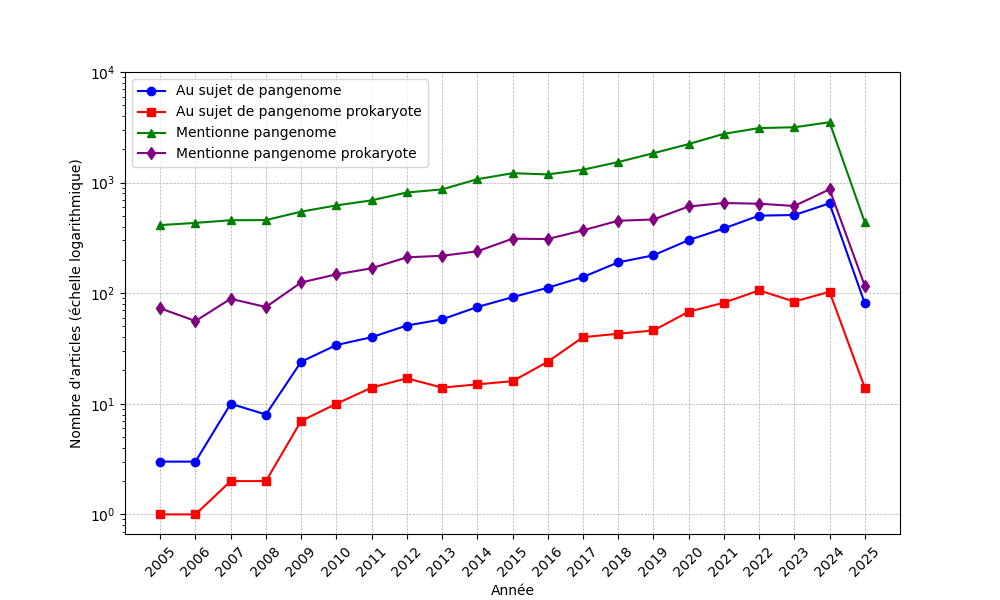
\includegraphics[width=\linewidth]{images/pangenomeCitation.png}
    \caption[Bibliométrie pangénome]{Nombre d'articles, référencé dans PubMed, par année, à propos de pangénome de 2004 au 10 février 2025. La courbe bleue représente le nombre d'articles contenant le terme pangénome dans le titre ou l'abstract : Query=("pan-genome"[Title/Abstract] OR "pangenome"[Title/Abstract] OR "pan-genome"[Title/Abstract]) AND (2004:2025[pdat]). La courbe rouge limite aux publications concernant les procaryotes : Query=("procaryote"[Title/Abstract] OR "bacteria"[Title/Abstract] OR "archeae"[Title/Abstract]) AND ("pan-genome"[Title/Abstract] OR "pangenome"[Title/Abstract] OR "pan-genome"[Title/Abstract]) AND (2004:2025[pdat]). La courbe verte représente tous les articles ou le terme pangénome est trouvé : Query=((pangenome) OR (pan genome)) OR (pan-genome) AND (2004:2025[pdat]). La courbe violette filtre les publications concernant les procaryotes : Query=(((procaryote) OR (bacteria)) OR (archeae)) AND (((pan-genome) OR (pangenome)) OR (pan genome)) AND (2004:2025[pdat]).}
    \label{fig:panCite}
\end{figure}

Le pangénome est une structure de données complexes qui peut contenir un ensemble d'informations. Notamment, à partir du pangénome, Tettelin \textit{et al.} propose de séparer les gènes en 2 catégories, les gènes "\textit{core}" commun à tous les génomes, des gènes "\textit{dispensable}" trouver dans un sous-ensemble de génomes. En généralisant, le pangénome permet de distinguer l'ensemble des séquences communes à tous les organismes, des variations présente chez certains groupes d'individus, voire spécifique à un organisme. De ce postulat a émergé l'idée de remplacer les génomes de références dans les bases de données par des pangénomes de références. Toutefois, ce changement de paradigme n'a pas encore été opéré, car il pose plusieurs questions. La première est la question de la représentation des pangénomes, nous aborderons les modèles et représentations des pangénomes, qui doit être visualisable par l'\oe il humain, tout en intégrant l'ensemble de l'information du pangénome. La seconde question est celle du stockage, les génomes sont généralement stockés sous forme de texte et relié à leurs informations dans des bases de données. Le pangénome est une structure plus complexe, qui n'est pas possible de stocker sous forme de texte. De plus, les bases de données contenant les pangénomes doivent pouvoir être interrogé de façon efficace. Étant donné l'augmentation du volume de données génomique dans les bases, il est également nécessaire que la base de données puissent être mise à jour régulièrement. La dernière question, essentiel, est : quelle méthode utiliser pour construire le pangénome ? Il faut tout d'abord définir les éléments qui constituent le pangénome, \textit{i.e.}, les gènes ou des k-mers pour les variants, ou encore des séquences d'ADN plus longues. Il faut ensuite connecter ces éléments, selon des critères pertinents. Enfin, il faut pouvoir donner un sens au pangénome et donc il faut pouvoir y appliquer des algorithmes pour l'analyser. Toutes ces questions n'ont pas encore trouvé de réponse consensus dans la communauté et aucune méthode n'a encore réussi à s'imposer comme solutions optimales. Trouvé une méthode globale est aussi un défi, car la pangénomique est appliqué dans de nombreux domaines de recherches, pour répondre à une grande diversité de question.

La pangénomique est largement utilisée dans de nombreux domaines. Le "Computational Pan-Genomics Consortium" met en avant son rôle dans le développement de solutions applicatives répondant à des problématiques communes à plusieurs disciplines \cite{the_computational_pan-genomics_consortium_computational_2018}. Elle bénéficie ainsi des avancées en phylogénie, métagénomique et intelligence artificielle.

En phylogénie, les méthodes de comparaison génomique à grande échelle et les techniques de construction d'arbres phylogénétiques ont été intégrées aux approches pangénomiques. En retour, la pangénomique permet une meilleure prise en compte des variations génétiques à l'échelle de l'ensemble des génomes, plutôt que de se limiter à un génome de référence, offrant ainsi une vision plus fine de la dynamique évolutive.

En métagénomique, les outils d’assemblage ont été adaptés pour affiner la reconstruction des pangénomes. Les algorithmes de \textit{binning}\footnote{Procédure de regroupement des contigs assemblé et d'assignation à un génome d'origine.} et de profilage génétique facilitent l’identification de clusters de gènes conservés et variables. En retour, la pangénomique enrichit l’analyse de la diversité génétique au sein des communautés microbiennes, dépassant ainsi la seule représentation de la diversité des génomes au sein d’un taxon.

L’intelligence artificielle joue également un rôle clé en améliorant l’annotation et la prédiction fonctionnelle des gènes. L’apprentissage automatique est appliqué à la pangénomique pour détecter des motifs génétiques pertinents, prédire des phénotypes et identifier des associations entre mutations et traits phénotypiques.

Ces méthodes, souvent développées pour d’autres disciplines, ont donc favorisé l’essor de la pangénomique en optimisant l’analyse des données, la reconstruction des génomes et l’interprétation des résultats.

La pangénomique se présente donc comme une solution à l'analyse de grand volume de données, à l'heure où le nombre de génomes disponible dans les banques augmentent de façon exponentielle, mais apporte aussi son lot de défis.

\subsection{Modélisation de la croissance des pangénomes}
\label{sec:croissance_pan}

Dans l'article original de Tettelin \textit{et al.}, les auteurs s'intéresse à la distribution \textit{core/dispensable} en fonction du nombre de génomes de \textit{Streptococcus agalactiae}\footnote{Bactérie du microbiote intestinale humain et animal, qui est également associé à des infections graves.} que contient le pangénome. Ils observent que lorsque le nombre de génomes augmente, la part de \textit{core genome} décroît de façon exponentielle. Ce résultat les amène à modéliser la croissance du \textit{core genomes} selon une équation exponentielle décroissante. Le modèle permet alors d'estimer la taille du \textit{core genome} pour un nombre de génomes en théorie infinie. Il est alors possible d'estimer la taille du \textit{core genome} d'une espèce à partir d'un échantillon de génome. 

À partir de ce modèle, il est également possible d'estimer la taille du pangénome, \textit{i.e.}, le nombre de gènes unique que contient le pangénome. Ils définissent alors 2 types de pangénomes en fonction de l'estimation de la taille : les pangénomes ouvert et les pangénomes fermés. Les pangénomes sont considérés comme ouverts lorsque le nombre de gènes ajouté au pangénome lors de l'ajout d'un nouveau génome, ne diminue pas avec l'ajout de nouveaux génomes. Le nombre de gènes est donc théoriquement infini pour un pangénome ouvert avec une infinité de génomes. Les pangénomes fermé quant à eux voit le nombre de nouveaux gènes progressivement diminué lors de l'ajout de nouveaux génomes. La courbe de prédiction permet d'identifier un plateau théorique du nombre maximal de familles que contiendra le pangénome avec un nombre de génomes infinis. Biologiquement, le pangénome ouvert est attendu pour les espèces sympatriques\footnote{Espèces vivant dans le même environnement que d'autres espèces.} et qui présentent un fort taux de transfert horizontaux, tandis que les espèces vivant dans des niches écologiques ou qui ont une faible capacité d'acquisition de gènes extérieurs vont avoir un pangénome fermé.

\begin{figure}[htbp]
    \centering
    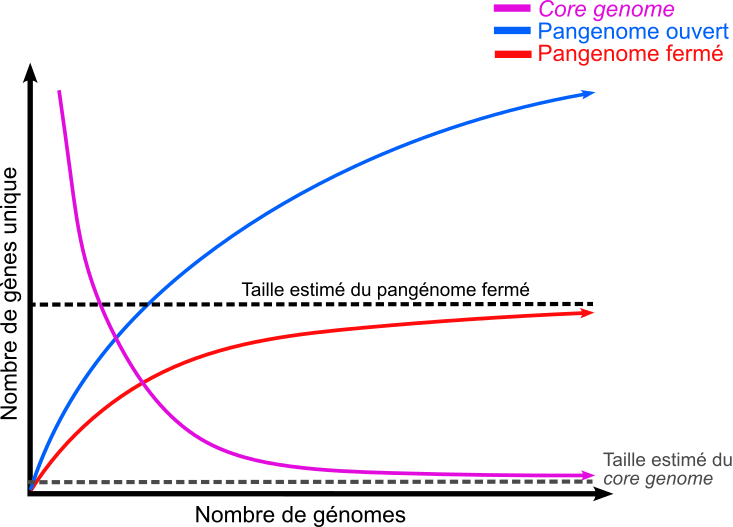
\includegraphics[width=0.7\linewidth]{images/panOpenClose.png}
    \caption[Schéma de croissance du pangénome]{Schéma de croissance du pangénome.}
    \label{fig:panOpenClose}
\end{figure}

Le modèle proposé par Tettelin \textit{et al.}, repose sur l'hypothèse que pour un nombre suffisant de génomes, le nombre de nouveaux gènes apporté par un génome devient constant à partir d'un certain nombre de génomes. Cette hypothèse implique alors que la taille du pangénome est infinie. Cette hypothèse sera questionnée par Hogg \textit{et al.} dans leur étude du pangénome de \textit{Haemophilus influenzae} \cite{hogg_characterization_2007}. Ils vont alors proposer une modélisation basée sur l'hypothèse que le pangénome est fini. Dans leur modèle, chaque gène est associé à une variable aléatoire de Bernoulli, dont la probabilité correspond à la fréquence du gène dans les génomes. Un génome est ainsi généré en observant ces variables : un gène est présent si l’essai est un succès, sinon il est absent. Bien que certains gènes ne soient pas indépendants en raison de structures comme les îlots génomiques, cette hypothèse est conservée pour simplifier le modèle. Les fréquences réelles des gènes étant inconnues, elles sont modélisées de manière probabiliste en répartissant les gènes en $K$ classes distinctes, chacune ayant une fréquence de présence spécifique. À partir de ce modèle, sur le pangénome de \textit{H. influenzae} avec $K=7$, la taille du pangénome est estimé à 5 000 gènes (contre 2 800 gènes dans les 13 génomes de bases). Ce modèle sera ensuite amélioré par Snipen \textit{et al.} \cite{snipen_microbial_2009}, qui proposeront une détermination automatique du nombre de classes $K$ et de la fréquence théorique des gènes pour chaque classe. Les modèles binomiaux propose une perspective dans laquelle la diversité en gènes est finie et qu'il existe un nombre de génomes suffisamment grand pour que tout le répertoire génique soit connu. Cette vision semble de prime abord logique, car le nombre de combinaisons possible de nucléotide ou d'acide aminé est fini. Pourtant, on peut y opposer que ce nombre, sans le calculer, semble démesuré et qu'il peut être considéré comme infini. De plus, les génomes évoluent continuellement et que de nouveaux gènes apparaissent sans cesse. L'utilisation des modèles binomiaux semble alors plus approprié à des espèces de niche, isolé et présentant un faible taux de transfert horizontaux.

En 2008, Tettelin \textit{et al.} vont proposer une nouvelle modélisation basée sur la loi de Heaps\footnote{Définit de manière empirique en linguistique, cette loi permet de décrire le nombre de mots d'une langue à partir d'un ensemble de documents.} \cite{tettelin_comparative_2008}. On estime le nombre $n$ de gènes distincts, en fonction du nombre $N$ de génomes étudiés, selon la relation :
\begin{equation}
    n=kN^\gamma, 0<\gamma<1,k\geq1
\end{equation}

Le paramètre $k$ est une constante de proportionnalité tandis que $\gamma$ reflète la tendance de la fonction. Ainsi, plus $\gamma$ est proche de 0 plus la croissance en gène distinct est lente, et plus $\gamma$ est proche de 1 plus la croissance est rapide (\autoref{fig:HeaplawGamma}).

\begin{figure}[htbp]
    \centering
    \subfloat[]{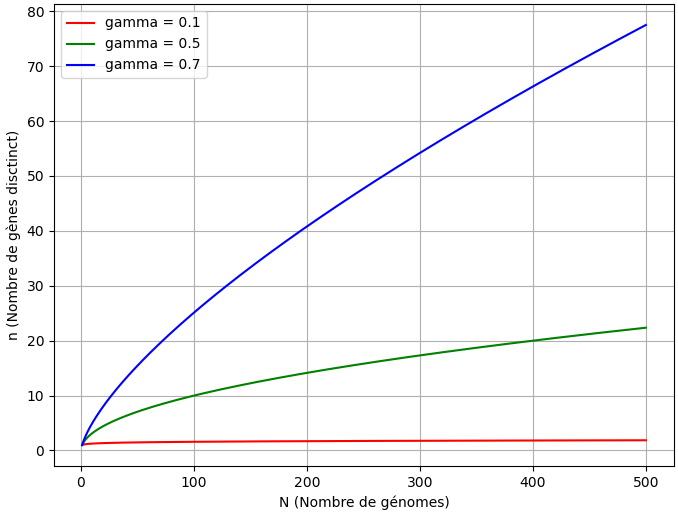
\includegraphics[width=0.48\linewidth]{images/HeapsLawgamma.png}
    \label{fig:HeaplawGamma}}
    \hfill
    \subfloat[]{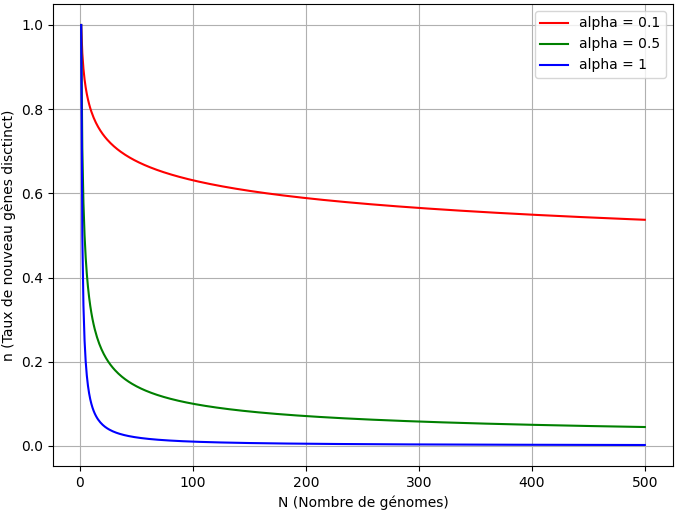
\includegraphics[width=0.48\linewidth]{images/HeapsLawAlpha.png}
    \label{fig:HeaplawAlpha}}
    \caption{Caption}
    \label{fig:Heaplaw}
\end{figure}

Selon la loi de Heap, le nombre de nouveau gènes découvert diminue à mesure que l'on ajoute des génomes. On peut formuler ceci selon l'équation : 

\begin{equation}
    p(n)=kN^{(\gamma-1)}=kN^{-\alpha}, \alpha=1-\gamma
\end{equation}

Ainsi, sur la \autoref{fig:HeaplawAlpha}, lorsque $0<\alpha<1$, le taux de nouveaux gènes décroit en ajoutant des génomes, sans jamais être nulle. Dans ce cas, le nombre de gènes distinct est croissant. Ce qui implique que si $0<\alpha<1$, le pangénome est ouvert. À partir d'un ensemble de génome, il est possible d'estimer k et $\alpha$ (ou $\gamma$) et donc de caractériser si le pangénome est ouvert. Si $\alpha\geq1$, alors le taux de nouveaux gènes atteint 0, ce qui correspond à un pangénome fermé. 

\subsection{Les différents types de pangénomes}

Les pangénomes peuvent être divisés en 2 catégories en fonction de l'unité choisit pour les construire. Le premier type, celui présenté par Tettelin \textit{et al.} \cite{tettelin_genome_2005}, utilise les gènes comme unité de base du pangénome (\autoref{fig:panType}.B). En regroupant les gènes par homologie (appelé famille de gènes, cf. \autoref{sec:fam}), il est possible d'obtenir la présence/absence de gènes similaire dans les génomes. Ces pangénomes ont l'avantage d'être moins couteux en ressources de calcul pour être construit. De plus, ils sont faciles à interpréter, car les gènes sont des unités déjà bien définies et parfois, ils sont même annotés fonctionnellement. Néanmoins, en utilisant les gènes, la méthode d'annotation à un impact important sur le pangénome et il est sensible aux erreurs d'annotation. De plus, les régions non codantes ne sont pas prises en compte dans cette approche. Enfin, les SNPs peuvent passer inaperçu après le regroupement, ainsi que les variants structuraux (SV).

L'autre type de pangénome est basé sur les séquences brutes des génomes. Cette approche plus récente, qui peut être associé à l'outil GenomeMapper \cite{schneeberger_simultaneous_2009}, permet d'identifier les parties similaires des parties variables à partir d'un alignement complet des séquences découpé en k-mers (\autoref{fig:panType}.C,D). Cette approche a l'intérêt de prendre en compte toute la diversité des génomes (codant, non codant, SNPs et SV). Toutefois, la construction de ces pangénomes est plus coûteuse en ressources. De plus, l'interprétation est plus complexe, car le pangénome n'est pas annoté au départ. Pour terminer, certaines méthodes de construction, utilise un génome de référence comme séquence de base (\autoref{fig:panType}.C), ce qui peut aussi introduire un biais.

\begin{figure}[htbp]
    \centering
    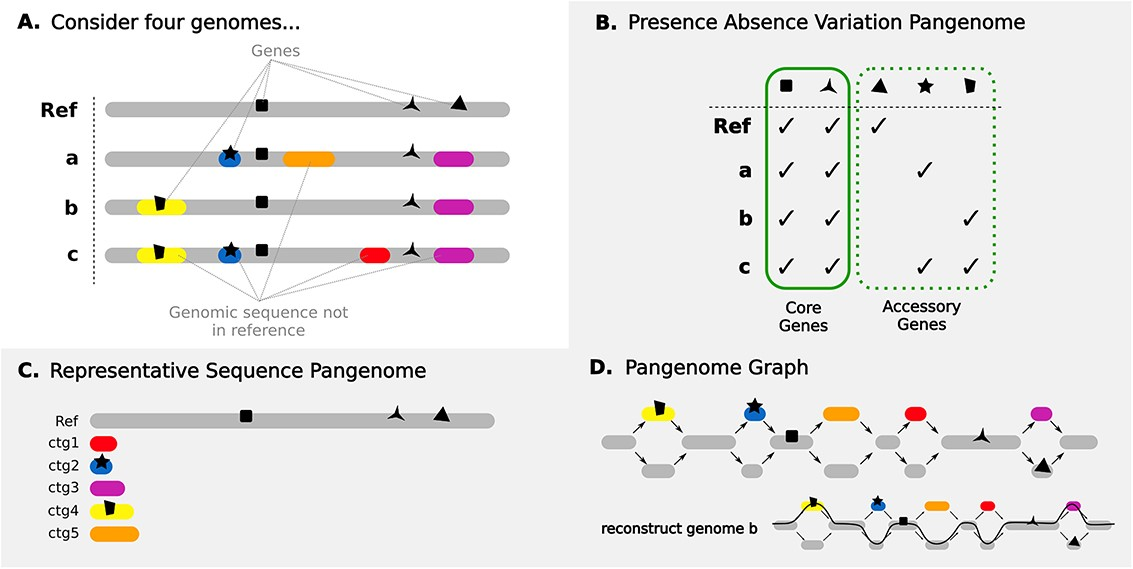
\includegraphics[width=0.8\linewidth]{images/pangenomeTypes.jpeg}
    \caption[Différents types de pangénomes]{Différents types de pangénomes. Extrait de \cite{matthews_gentle_2024}}
    \label{fig:panType}
\end{figure}
